Sabe-se que algoritmos de AM necessitam de quantidade significante de dados, preferencialmente sem muitos ruídos, para serem executados de forma a obter um bom desempenho \cite{marsland}. Portanto, visando a consolidação de uma base de dados própria que se adeque a solução proposta e que diminua a sobrecarga de processamento necessária para o treinamento do modelo, fez se necessário um pré-processamento das imagens contidas no conjunto de dados disponibilizado pelo IAPR.

Foi necessária a adaptação das imagens de forma a seguir o processo de aprendizado ilustrado na Figura \ref{fig:esquema-solucao}. Para isto, foi feita a combinação de cada assinatura genuína de um autor com ela mesma e suas outras assinaturas genuínas, a fim de criar exemplos genuínos, e também a combinação dessa assinatura com cada assinatura forjada do mesmo autor, criando assim os exemplos rotulados como forjados. Todas as imagens obtidas dessas combinações foram utilizadas como exemplos para o processo de treinamento, validação e teste do modelo proposto.

O processo de combinação dessas imagens foi concluído em três etapas. Na primeira etapa do processo, ambas as imagens foram redimensionadas para um tamanho de $256 \times 256$ \emph{pixels}. Em seguida, as imagens foram concatenadas verticalmente com a intenção de formar uma única imagem de $256 \times 512$ \emph{pixels}. Por fim, a imagem resultante foi redimensionada novamente em um tamanho de $256 \times 256$ \emph{pixels} e transformada para um espaço de cores em escala de cinza, com a intenção de padronizar todas as entradas recebidas pelas CNNs.

% Escrever algo sobre como foi atingida a quantidade de exemplos atual?

Devido a desproporção no número de exemplos genuínos e forjados e considerando que para alguns indivíduos o conjunto de dados original não possuia assinaturas forjadas, apenas genuínas, foi necessário consolidar bases de dados diferentes considerando três abordagens distintas, visando um melhor aproveitamento dos exemplos disponíveis e a consideração de diferentes percentuais de exemplos. Como pode ser visualizado na Figura \ref{fig:divisao-dados}, em todas as abordagens a proporção de dados separados para as etapas treinamento, teste e validação foi a mesma, aproximadamente $70\%$ para treinamento, aproximadamente $20\%$ para teste e aproximadamente $10\%$ para validação.

\begin{figure}[h!]
	\centering
	\caption{Detalhamento da quantidade de exemplos por finalidade e por abordagem.}
	\subfloat[Abordagem 1\label{subfig:approach1}]{%
	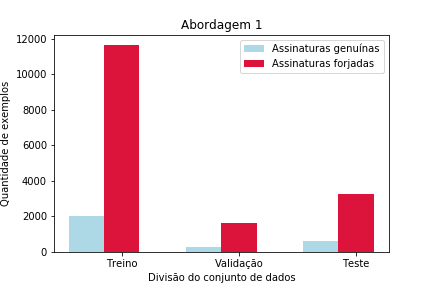
\includegraphics[width=0.5\textwidth]{imgs/approach1}
	}
	\subfloat[Abordagem 2\label{subfig:approach2}]{%
	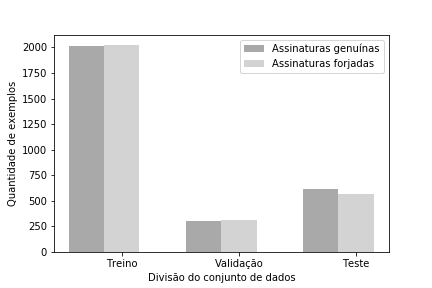
\includegraphics[width=0.5\textwidth]{imgs/approach2}
	}
	\hfill
	\subfloat[Abordagem 3\label{subfig:approach3}]{%
	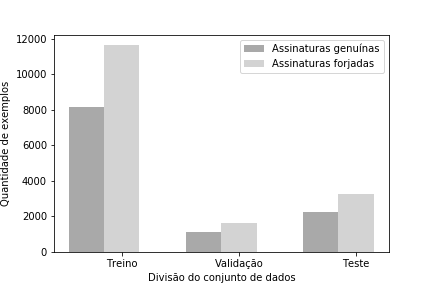
\includegraphics[width=0.5\textwidth]{imgs/approach3}
	}
	\label{fig:divisao-dados}
\end{figure}

Na primeira abordagem, foram considerados apenas os exemplos nos quais os indivíduos possuíam assinaturas genuínas e forjadas, sem se importar com a quantidade de exemplos para cada classe, criando assim uma base de dados com uma característica desbalanceada. Entretanto, para a segunda abordagem, foram retirados alguns exemplos de assinaturas forjadas de forma pseudoaleatória, a fim de criar uma base de dados balanceada. Por fim, na terceira abordagem, além de se utilizar todos os dados da primeira abordagem, utilizou-se também os exemplos genuínos de indivíduos que não possuíam assinaturas forjadas, criando desta forma uma base de dados com uma característica \emph{quasi}-balanceada. Uma descrição mais detalhada da composição dos dados em cada uma das abordagens pode ser visualizado na Tabela \ref{tab:divisao-dados}.

% Processo de obtenção do exemplo que será dado como entrada às CNNs.
% Descrição das abordagens
% O processo de separação dos dados de treinamento, validação e teste.

\begin{table}[h!]
	\centering
	\caption{Quantitativo de exemplos de cada classe por finalidade dos dados na tarefa de AM.}
	\label{tab:divisao-dados}
\resizebox{\textwidth}{!}{
	\begin{tabular}{c c c c c c c c}
		\toprule
		\textbf{Abordagem} & \textbf{Característica} & \textbf{Tipo de Exemplo} & \textbf{Treino} & \textbf{Validação} & \textbf{Teste} & \textbf{Total} & \textbf{Proporção}\\
		\midrule
		\multirow{2}{*}{1} & \multirow{2}{*}{Dados desbalanceados} & Genuíno & 2.011 & 299 & 618 & 2.928 & $15\%$ \\
    &  & Forjado & 11.649 & 1.648 & 3.237 & 16.534 & $85\%$\\
     \midrule
    \multirow{2}{*}{2} & \multirow{2}{*}{Dados balanceados} & Genuíno & 2.011 & 299 & 618 & 2.928 & $50\%$  \\
    &  & Forjado & 2.024 & 308 & 569 & 2.901 & $50\%$ \\
		 \midrule
		\multirow{2}{*}{3} & \multirow{2}{*}{Dados \emph{quasi}-balanceados} & Genuíno & 8.131 & 1.134 & 2.257  & 11.522 & $41\%$\\
		 & & Forjado & 11.649 & 1.648 & 3.237 & 16.534 & $59\%$\\
		\bottomrule
	\end{tabular}}
\end{table}
